\section{Generating Correlated Poisson Variables}\label{ch:generate_correlated_poisson}
In presenting the simulation procedure, it is necessary to discuss the method for generating correlated Poisson processes. I use a method similar to the ones discussed by \cite{A8} to generate multivariate Poisson variables with the desired correlations. 

Here, I will discuss the general procedure used to generate a $d$-dimensional multivariate Poisson variable. The goal is to generate random variables $N_1, N_2, \ldots, X_d$ with means $\lambda_1, \lambda_2, \ldots, \lambda_{d}$ and correlations defined by the $d$x$d$ matrix $\sigma$ where each variable $N_i$ has a marginal distribution that is the same as the marginal distribution as a Poisson variable with mean $\lambda_i$. That is, $P(X_i = a) = f_i(a)$, where $f_i$ is the probability mass function of a Poisson variable with mean $\lambda_i$.

To do so, I make use of a copula. A copula is defined as any joint probability distribution function where each marginal distribution is uniformly distributed \cite{B1}. That is, 
$$C(u): [0,1]^d \to [0,1]$$ 
is a copula if $C(0, 0, \ldots, 0) = 0$ and $C(1, 1, u_i, 1, \ldots, 1) = u_i$ and $u_i \in [0,1]$ for all $i$. I will use the Gaussian copula as described in \cite{A8} where

$$ C_\sigma^{Gaussian}(u_1, u_2, \ldots, u_d) = \Phi_\sigma(\Phi^{-1}(u_1), \Phi^{-1}(u_2), \ldots,  \Phi^{-1}(u_d))$$

where $\Phi$ is the cumulative distribution function for a standard random normal variable and $\Phi_\sigma$ is the cumulative distribution function for a random multivariate normal vector with mean $0$, variance $1$, and correlation matrix $\sigma$. I can generate $u$ by first generating a multivariate normal random variable $Y = (Y_1,Y_2, \ldots, Y_d)$ with correlation matrix $\sigma$ and setting $(u_1, u_2, \ldots, u_d) = (\Phi(y_1), \Phi(y_2), \ldots,  \Phi(y_d))$. I then pair it with a copula that has marginal Poisson distributions. Namely,

$$ C^{Poisson}(F_1(x_1), F_2(x_2), \ldots, F_d(x_d))$$ where $F_i$ is the discrete cumulative distribution function for a Poisson random variable with rate $\lambda_i$. I can then set

$$(n_1, n_2, \ldots, n_d) = (F^{-1}_1(u_1), F^{-1}_2(u_2), \ldots, F^{-1}_d(u_d))$$

To implement $F^{-1}_i(u_i)$, I will use the inverse transform method described in \cite{B1}:
\newline

\begin{algorithm}[H]
\SetAlgoLined
\caption{Inverse Transform Method for Poisson Variable With Rate $\lambda$ and input $u$}
 $i = 0$\;
 $p = e^{-\lambda}$\;
 $F = p$\;
 \While{$u >= F$}{
  $p = \lambda p / (i + 1)$ \;
  $F = F + p$ \;
  $i = i + 1$ \;
 }
 return $i$ \;
\end{algorithm}

Each $x_i$ will have a marginal Poisson distribution with rate $\lambda_i$ and $x$ will approximately have correlation matrix $\sigma$. Table \ref{tab:experimental_correlation} shows the performance of this method. For each desired correlation we generate 10000 pairs $(x_1,x_2)$ that have means $1$ and have a joint Poisson distribution (see Listing \ref{correlated-poisson}). $x_1$ and $x_2$ have the correct means for each correlation level. For positive correlations, the actual correlation is slightly below the desired correlation (less than 0.1 difference). For negative correlations, the actual correlation is slightly above the desired correlation for smaller magnitudes and deviates more significantly at higher magnitudes. In practice, our correlation matrix contains values that range from small negative small correlations to large positive correlations (see Tables \ref{tab:pos_pos_corr_tab}, \ref{tab:pos_neg_corr_tab}, and \ref{tab:neg_neg_corr_tab}), so this method generates Poisson arrivals that follow $\sigma$ relatively closely. It may be possible to generate arrivals that more closely follow given correlations, but this method provides acceptable performance given our data.

\begin{table}
\label{tab:experimental_correlation}
\centering
\caption{Actual vs. Desired Correlation Using Gaussian Copula, $n=10000$}
\begin{tabular}{l|l|l|l}
Desired Correlation & $\bar{x_1}$ & $\bar{x_2}$ & Actual Correlation  \\ 
\hline
-1                  & 0.995                           & 1.009                           & -0.735              \\
-0.9                & 0.997                           & 0.997                           & -0.682              \\
-0.8                & 1.01                            & 0.985                           & -0.616              \\
-0.7                & 0.987                           & 1.003                           & -0.543              \\
-0.6                & 0.99                            & 1.014                           & -0.472              \\
-0.5                & 0.998                           & 1.002                           & -0.405              \\
-0.4                & 1.016                           & 0.988                           & -0.308              \\
-0.3                & 1.003                           & 1.005                           & -0.236              \\
-0.2                & 1.001                           & 1.007                           & -0.163              \\
-0.1                & 0.998                           & 1.018                           & -0.086              \\
0                   & 1.014                           & 0.986                           & 0.016               \\
0.1                 & 0.976                           & 0.992                           & 0.062               \\
0.2                 & 0.994                           & 0.986                           & 0.162               \\
0.3                 & 0.995                           & 1.002                           & 0.246               \\
0.4                 & 1.006                           & 1.004                           & 0.371               \\
0.5                 & 1                               & 0.997                           & 0.433               \\
0.6                 & 0.987                           & 1.001                           & 0.522               \\
0.7                 & 1.007                           & 1.007                           & 0.616               \\
0.8                 & 0.993                           & 0.986                           & 0.727               \\
0.9                 & 1.01                            & 1.008                           & 0.829               \\
1                   & 0.997                           & 0.997                           & 1                  
\end{tabular}
\end{table}

\section{Backwards Simulation} \label{ch:backwards_simulation}

Section \ref{ch:generate_correlated_poisson} shows how to generate correlated Poisson variables with specified means and correlations. The correlation matrix $\sigma$ reflects correlations between numbers of events in a time period of length $t$, so we can generate numbers of events using means equal to $\lambda^+_k t$ and $\lambda^-_k t$ for positive and negative events. Given the numbers of arrivals, a method called backwards simulation can be used to simulate the times of events (described in \cite{A7}). 

Backwards simulation utilizes the fact that conditioned on the number of arrivals in a Poisson process in a time period $t$ being equal to $n$, these arrivals are distributed uniformly across $[0,t]$. Using this method, I can generate arrivals over a larger time period $T$ (i.e. $T = 10t$) by simulating arrivals in smaller chunks of size $t$. An algorithm is presented below for simulating arrivals over a time period $T$, with the arrivals following a multivariate Poisson process of dimension $d$, average rates $\lambda_i, i = 1, \ldots, d$ and correlation matrix $\sigma$. It returns a list of events $E$ whose entries $(i,c,\tau)$ are the type of event, size, and time respectively:

\begin{algorithm}[H]
\label{alg:backwards_simulation}
\SetAlgoLined
\caption{Backwards Simulation Method for Poisson Arrivals in time $T$}
 $i = 0$\;
 $E = []$;
 
 \While{$it < T$}{
  Generate $(n_1, n_2, \ldots, n_d)$ using procedure described in section \ref{ch:generate_correlated_poisson};
  
  \For{$j = 1, \ldots, d$} {
  
    \For{$n = 1, \ldots, n_j$} {
        Generate a uniform random variable $u \in [it, (i+1)t)$;
        Generate a variable $y$ that is distributed exponentially with mean $\mu_j$
        Append $(j,y,u)$ to $E$;
    }
  
  }
 }
 return $E$ \;
\end{algorithm}

Sample arrivals for our LOB are show in Figures \ref{fig:bid_events_graphs} and \ref{fig:ask_events_graphs}. The magnitude of the events are generated according to the method described in \ref{ch:event_sizes}. Positive events are shown in blue while negative events are shown in orange.

\begin{figure}
\centering
\caption{Bid Arrivals over $T$ = 600 seconds}
\begin{tabular}{cc}
\hline
\subf{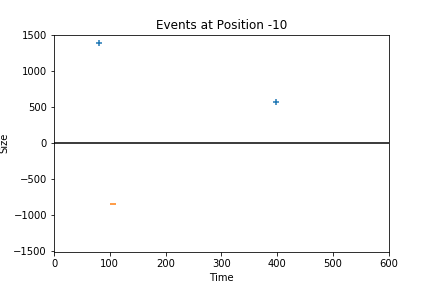
\includegraphics[width=60mm]{Figures/Events/events-10.png}}
{}
&
\subf{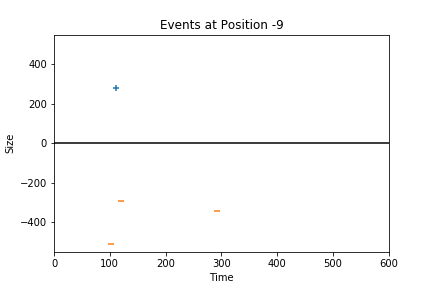
\includegraphics[width=60mm]{Figures/Events/events-9.png}}
{}
\\
\subf{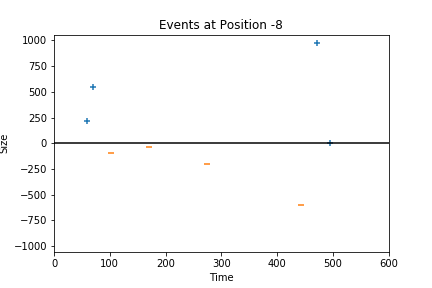
\includegraphics[width=60mm]{Figures/Events/events-8.png}}
{}
&
\subf{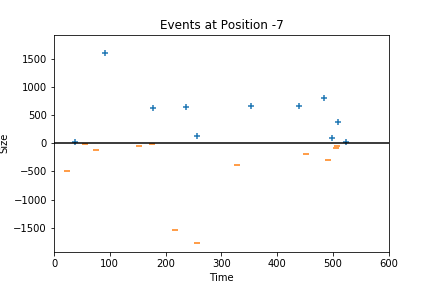
\includegraphics[width=60mm]{Figures/Events/events-7.png}}
{}
\\
\subf{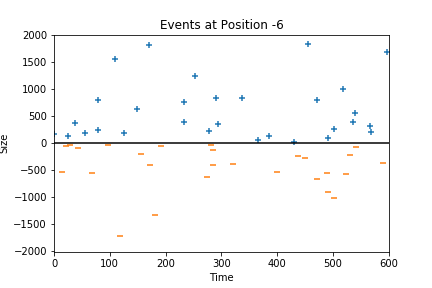
\includegraphics[width=60mm]{Figures/Events/events-6.png}}
{}
&
\subf{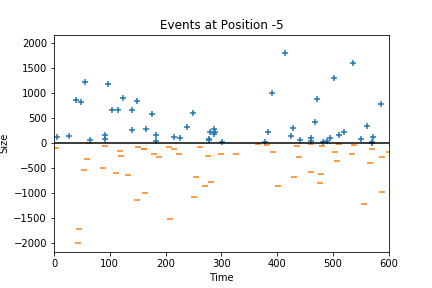
\includegraphics[width=60mm]{Figures/Events/events-5.png}}
{}
\\
\subf{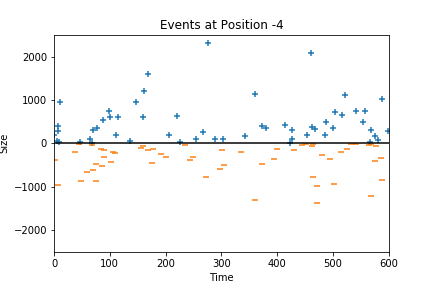
\includegraphics[width=60mm]{Figures/Events/events-4.png}}
{}
&
\subf{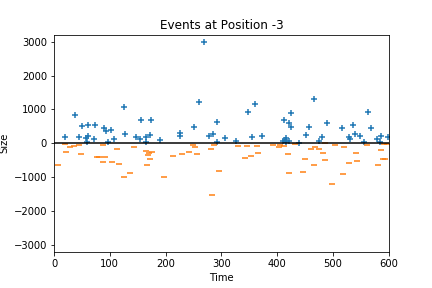
\includegraphics[width=60mm]{Figures/Events/events-3.png}}
{}
\\
\subf{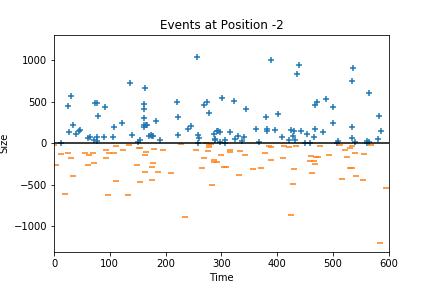
\includegraphics[width=60mm]{Figures/Events/events-2.png}}
{}
&
\subf{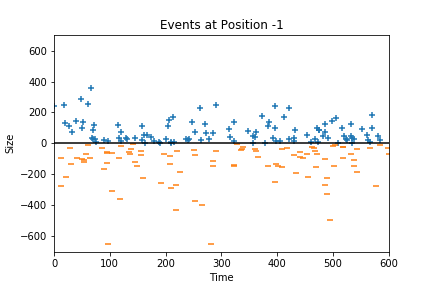
\includegraphics[width=60mm]{Figures/Events/events-1.png}}
{}
\\
\hline
\end{tabular}
\label{fig:bid_events_graphs}
\end{figure}

\begin{figure}
\centering
\caption{Ask Arrivals over $T$ = 600 seconds}
\begin{tabular}{cc}
\hline
\subf{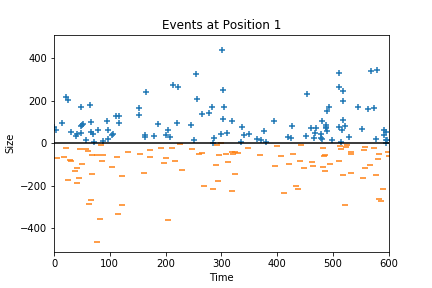
\includegraphics[width=60mm]{Figures/Events/events1.png}}
{}
&
\subf{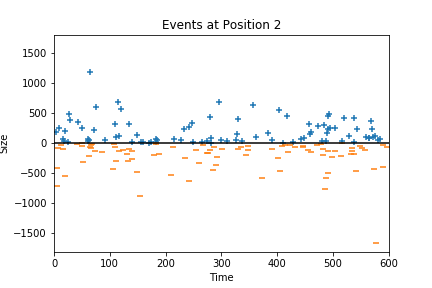
\includegraphics[width=60mm]{Figures/Events/events2.png}}
{}
\\
\subf{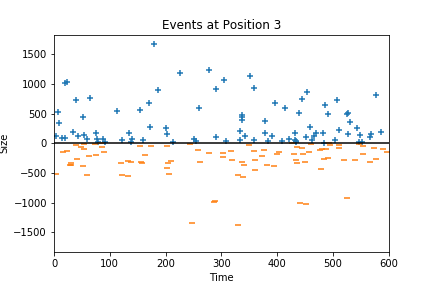
\includegraphics[width=60mm]{Figures/Events/events3.png}}
{}
&
\subf{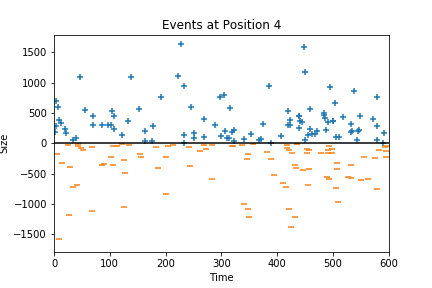
\includegraphics[width=60mm]{Figures/Events/events4.png}}
{}
\\
\subf{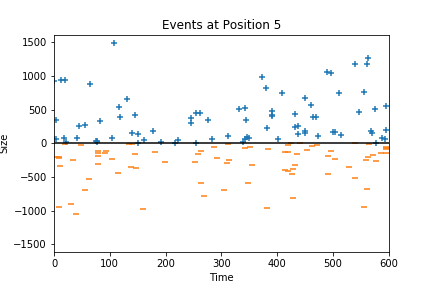
\includegraphics[width=60mm]{Figures/Events/events5.png}}
{}
&
\subf{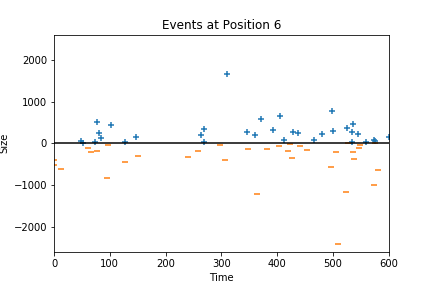
\includegraphics[width=60mm]{Figures/Events/events6.png}}
{}
\\
\subf{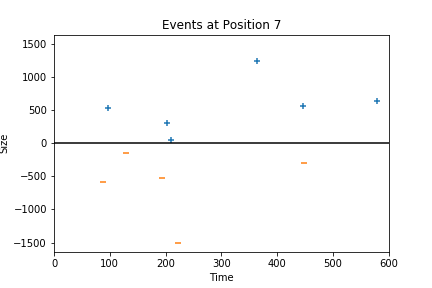
\includegraphics[width=60mm]{Figures/Events/events7.png}}
{}
&
\subf{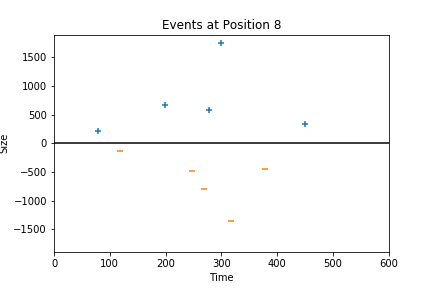
\includegraphics[width=60mm]{Figures/Events/events8.png}}
{}
\\
\subf{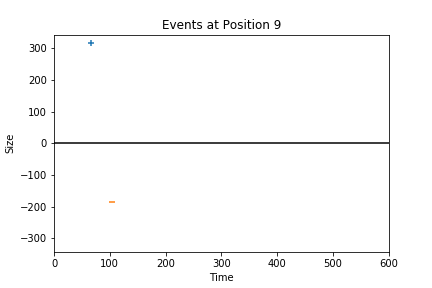
\includegraphics[width=60mm]{Figures/Events/events9.png}}
{}
&
\subf{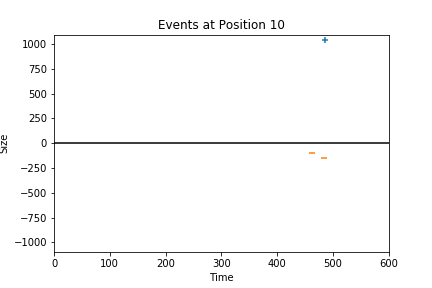
\includegraphics[width=60mm]{Figures/Events/events10.png}}
{}
\\
\hline
\end{tabular}
\label{fig:ask_events_graphs}
\end{figure}

\section{Simulation Algorithm} \label{ch:simulation_algorithm}

The actions of the agent can now be incorporated into the simulation. I assume that the agent needs to buy at least $V$ units in a time period $T$ and submits orders of the form $(a,\tau)$ which indicates a market buy order for amount $a$ at time $\tau$. At the end of the time period, if $A$ units have not been bought, then the trader makes a market order for the remainder of the inventory. External events on the order book are generated using the algorithm described in section \ref{ch:backwards_simulation}, and the reference price is updated as described in \ref{ch:queue_model}. The agent's market buys are executed at the best available price, and the simulation returns a list of executed trades of the form $(p,a,\tau)$, which contains the price, amount, and time of the trade.

See Listing \ref{code:simulation} for the code written to perform this simulation.

\begin{algorithm}[H]
\SetAlgoLined
\caption{Simulation of Order Book: Setup and Input}
Let $p_{ref}$ be the starting reference price ;

Let $L$ be the initial LOB at time $0$. Let $L_p$ be the volume at price $p$ ;

Let $v$ be the amount of inventory filled ;

Let $O$ be the trades executed ;

Let $\Theta$ be the list of orders of the form $(a,\tau)$ If $\sum{a} < V$, append $(V - \sum{a}, T)$ to $\Theta$;

Generate $E$ using Algorithm \ref{alg:backwards_simulation} $E$ contains events of form $(k,c,\tau)$ where $k$ is the position in relation to the reference price, $c$ is the change, and $\tau$ is the time ;

Sort $\Theta$ and $E$ by $\tau$ ;


Return $O$ ;
\end{algorithm}

\begin{algorithm}[H]
\SetAlgoLined
\caption{Simulation of Order Book: Tracking Market Orders}
Proceed through $\Theta$ and $E$ in time order. 

\While{$\tau <= T$ and $v < V$} {
    \If {\text{event of form} $(k,c,\tau)$} {
        convert $k$ to price $p$ ;
        \If {$c > 0$} {
            $L_p \leftarrow L_p + c$ ;
        }
        \Else {
            \If {\text{Best bid or best ask}} {
                Let $\eta = c$;
                \While {$\eta < 0$} {
                    $L_p \leftarrow max(0,L_p + \eta)$ ;
                    
                    $\eta \leftarrow \eta + max(L_p, -\eta)$ ;
                    
                    Set $p$ to be the next best price ;
                }
            }
            \Else {
                $L_p \leftarrow max(0,L_p + c)$ ;
            }
        }
    }
    \If {\text{order of form} $(a,\tau)$} {
        Let $p$ be the best ask ;
        Let $\eta = c$ ;
        \While {$\eta < 0$} {
            $L_p \leftarrow max(0,L_p + \eta)$ ;
            
            Append $(p,max(L_p, -\eta), \tau)$ to $O$ ;

            $\eta \leftarrow \eta + max(L_p, -\eta)$ ;
            
            $p \leftarrow p + 1$ ;
        }
    }
}

Return $O$ ;
\end{algorithm}







